\documentclass[12pt]{article}
\usepackage{graphicx}
\usepackage[margin=30mm, paper = a4paper]{geometry}
\usepackage{minted, caption}
\usepackage{subcaption}
\usepackage{multicol}

\title{Basic MySQL Operations}
\author{Md Tajim An Noor}
\date{}
\setlength{\columnseprule}{1pt}
\setlength{\columnsep}{2cm}
\begin{document}
\vspace*{\fill}
\begin{center}

    \emph{Heaven's Light is Our Guide} \\
    \textbf{Rajshahi University of Engineering and Technology} \\

    \begin{figure}[h]
        \centering
        
\includegraphics[scale=.34]{images/RUET_logo.png}
        \label{fig:ruet_logo}
    \end{figure}
    \vspace{5mm}

    \textbf{Course Code}\\
    ECE 2216\\
    \vspace{3mm}
    \textbf{Course Title}\\
    Database Systems Sessional

    \vspace{5mm}
    \textbf{Experiment Date:} October 15, 2023,\\
    \textbf{Submission Date:} November 5, 2023\\

    \vspace{5mm}
    \textbf{Lab Report 3:} Creating a database and doing operations on it using SQL\\

    \vspace{15mm}

    \begin{tabular}{c|c}
        \textbf{Submitted to} & \textbf{Submitted by} \\
        Md. Robiul Islam      & Md. Tajim An Noor     \\
        Assistant Professor   & Roll: 2010025         \\
        Dept of ECE, Ruet     &                       \\
    \end{tabular}

\end{center}
\vspace*{\fill}

\pagebreak

\tableofcontents

\maketitle

\section{Tools Used}
\begin{itemize}
    \item MySQL
    \item VS Code - as an IDE to use SQL
    \item MacTeX -\LaTeX  compiler
    \item VS Code with LaTeX workshop extension as a text editor
\end{itemize}


\section{Process}
The task is to create two tables in a database and then do some operations on the database using sub-query, Group By operations. The first table, Order, has the columns  ord\_date, purch\_amt, ord\_date, customer\_id, salesman\_id. The second one, named Customer, has the columns customer\_id, cust\_name, city, grade, salesman\_id.

\subsection{SQL Codes:}

\subsubsection*{Creating both tables and inserting data.}
\subsubsection*{Code:}
\begin{multicols}{2}{|}
    \begin{minted}[linenos,breaklines,breakanywhere]{mysql}
--creating the 1st table and adding info
CREATE TABLE ProductOrderDetailsLR3.Order(
    ord_no int Auto_Increment Primary Key,
    purch_amt decimal(6, 2),
    ord_date Date,
    customer_id int,
    salesman_id int -- )
    INSERT INTO
        ProductOrderDetailsLR3.Order (
            -- ord_no,
            purch_amt,
            ord_date,
            customer_id,
            salesman_id2
        )
    VALUES
        (
            70001,
            '150.5',
            '2012-10-05',
            3005,
            5002
        );

(2480.4, '2012-10-10', 3009, 5003),
(110.5, '2012-08-17', 3009, 5003),
(2400.6, '2012-07-27', 3007, 5001);

(70007, 948.5, '2012-09-10', 3005, 5002);

(5760, '2012-09-10', 3002, 5001),
(270.65, '2012-09-10', 3001, 5005),
(1983.43, '2012-10-10', 3004, 5006),
(75.29, '2012-08-17', 3003, 5007),
(250.45, '2012-06-27', 3008, 5002),
(3045.6, '2012-04-25', 3002, 5001);

-- creating the 2nd table and adding info

CREATE TABLE ProductOrderDetailsLR3.Customer(
    customer_id int Auto_Increment Primary Key,
    cust_name varchar(40),
    city varchar(40),
    grade int,
    ord_date Date,
    salesman_id int
-- )
ALTER TABLE
    ProductOrderDetailsLR3.Customer drop column ord_date;
INSERT INTO
    ProductOrderDetailsLR3.Customer (cust_name, city, grade, salesman_id)
VALUES
(
    3001,
    'Brad Guzan',
    'London',
    null,
    5005
);
(
    'Nick Romando',
    'New York',
    100,
    5001
),
(
    'Jozy Altidor',
    'Moscow',
    200,
    5007
).
-- To save space, some entries are shown.
    \end{minted}
\end{multicols}

\vspace{10mm}


\subsubsection{Calculate total purchase amount of all orders. Return total purchase amount.}
\subsubsection*{Code:}
\begin{minted}[breaklines, linenos]{mysql}
SELECT
    SUM(purch_amt) as "Total Purchase Amount"
FROM
    ProductOrderDetailsLR3.Order 
\end{minted}
\vspace{10mm}

\subsubsection{Count the number of unique salesperson. Return number of salesperson.}
\subsubsection*{Code: }
\begin{minted}[breaklines, linenos]{mysql}
SELECT
    salesman_id as "Salesperson",
    Count(*)
from
    ProductOrderDetailsLR3.Order
Group by
    salesman_id    
\end{minted}

\vspace{10mm}

\subsubsection{Find the highest grade of customers in each city. Return city, maximum grade.}
\subsubsection*{Code: }

\begin{minted}[breaklines, breakanywhere, linenos]{mysql}
SELECT
    city as City,
    grade as "Highest Grade"
FROM
    ProductOrderDetailsLR3.Customer Cust
WHERE
    grade = (
        SELECT
            max(grade)
        FROM
            ProductOrderDetailsLR3.Customer
        WHERE
            city = cust.city
        group by
            city
    );
\end{minted}

\vspace{10mm}

\subsubsection{Find the highest purchase amount ordered by each customer. Return customer ID, maximum purchase amount.}
\subsubsection*{Code:}

\begin{minted}[breaklines, linenos]{mysql}
SELECT
    customer_id as "Customer ID",
    purch_amt as "Max Purchase Amount"
FROM
    ProductOrderDetailsLR3.Order Cust
WHERE
    purch_amt = (
        SELECT
            max(purch_amt)
        FROM
            ProductOrderDetailsLR3.Order
        WHERE
            customer_id = Cust.customer_id
    )
Order by
    customer_id
\end{minted}



\vspace{10mm}

\subsubsection{Find the highest purchase amount ordered by each customer on a particular date. Return order date and highest purchase amount.}
\subsubsection*{Code: (Using sub-query)}
\begin{minted}[breaklines, linenos]{mysql}
SELECT
    ord_date as "Order Date",
    purch_amt as "Purchased Max Amount"
FROM
    ProductOrderDetailsLR3.Order Ord
WHERE
    purch_amt = (
        SELECT
            max(purch_amt)
        FROM
            ProductOrderDetailsLR3.Order
        WHERE
            ord_date = ord.ord_date
    )
Order by
    ord_date

    SELECT
    ord_date as "Order Date",
    max(purch_amt) as "Purchased Max Amount"
from
    ProductOrderDetailsLR3.Order
Group by
    ord_date
Order by
    ord_date
\end{minted}
\subsubsection*{Code: (Using GROUP BY clause)}
\begin{minted}[breaklines, linenos]{mysql}
SELECT
    ord_date as "Order Date",
    max(purch_amt) as "Purchased Max Amount"
from
    ProductOrderDetailsLR3.Order
Group by
    ord_date
Order by
    ord_date
\end{minted}



\vspace{10mm}

\subsubsection{Determine the highest purchase amount made by each salesperson on 2012-08-17. Return salesperson ID and purchase amount.}
\subsubsection*{Code:}
\begin{minted}[breaklines, linenos]{mysql}
SELECT
    salesman_id as "Salesperson ID",
    max(purch_amt) as "Purchased Max Amount",
    ord_date as "Ordered on"
from
    ProductOrderDetailsLR3.Order
WHERE
    ord_date = "2012-08-17"
Group by
    salesman_id
Order by
    salesman_id
\end{minted}

\vspace{13mm}

\subsubsection{Find the highest order \(purchase\) amount by each customer on a particular date. Filter the result by highest order purchase amount above 2000. Return customer ID, order date, highest purchase amount.}
\subsubsection*{Code:}
\begin{minted}[breaklines, linenos]{mysql}
SELECT
    customer_id as Customer,
    ord_date as "Order Date",
    max(purch_amt) as "Max ordered on date"
from
    ProductOrderDetailsLR3.Order
WHERE
    purch_amt > 2000
group by
    customer_id,
    ord_date
\end{minted}

\vspace{10mm}

\section{Output}
\captionsetup{justification=centering}
\begin{figure}[htbp!]
    \begin{subfigure}{1\textwidth}
        \centering
        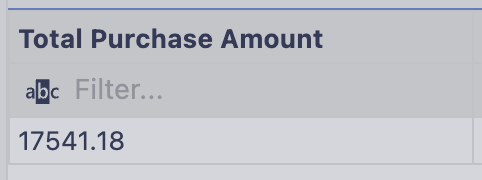
\includegraphics[width=\linewidth]{images/output/q1.png}
        \caption*{The person who is the top of the organization (i.e. reports to no one)}
        \label{fig:q1}
    \end{subfigure}
    \vspace*{20mm}
    \begin{subfigure}{.3\textwidth}
        \centering
        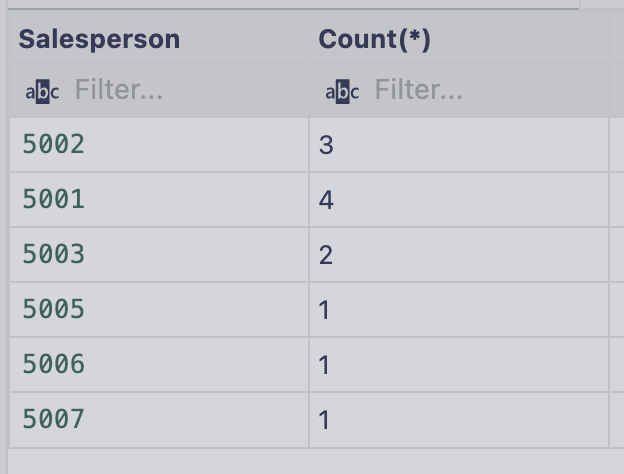
\includegraphics[width=.6\linewidth]{images/output/q2.png}
        \caption*{Difference in days between the most recent and oldest order date in Orders file.}
        \label{fig:q2}
    \end{subfigure}
    \begin{subfigure}{.3\textwidth}
        \centering
        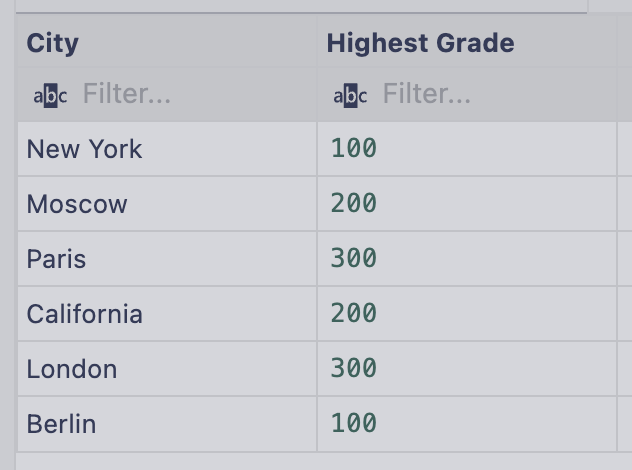
\includegraphics[width=.6\linewidth]{images/output/q3.png}
        \caption*{Total value of  payments received in July 2004.}
        \label{fig:q3}
    \end{subfigure}
    \begin{subfigure}{.3\textwidth}
        \centering
        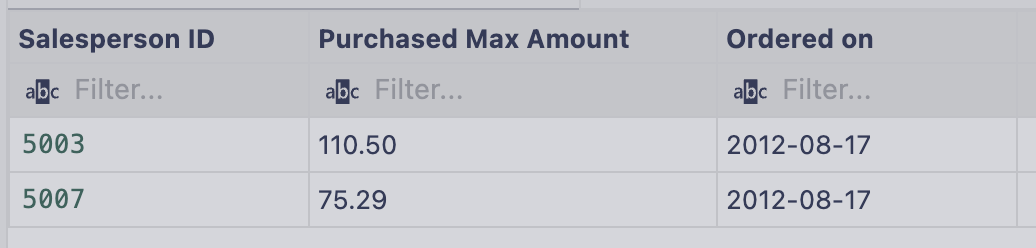
\includegraphics[width=.6\linewidth]{images/output/q6.png}
        \caption*{The number of orders ‘On Hold’ for each customer.}
        \label{fig:q6}
    \end{subfigure}

    \begin{subfigure}{\textwidth}
        \centering
        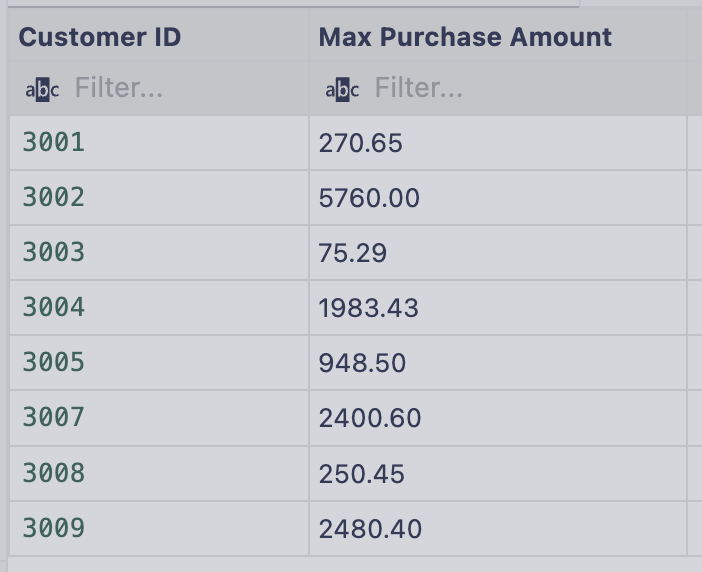
\includegraphics[width=.5\linewidth]{images/output/q4.png}
        \caption*{Profit generated by each sales representative based on the orders from the customers they serve. Sorted by profit generated descending.}
        \label{fig:q4}
    \end{subfigure}
    \begin{subfigure}{.5\textwidth}
        \centering
        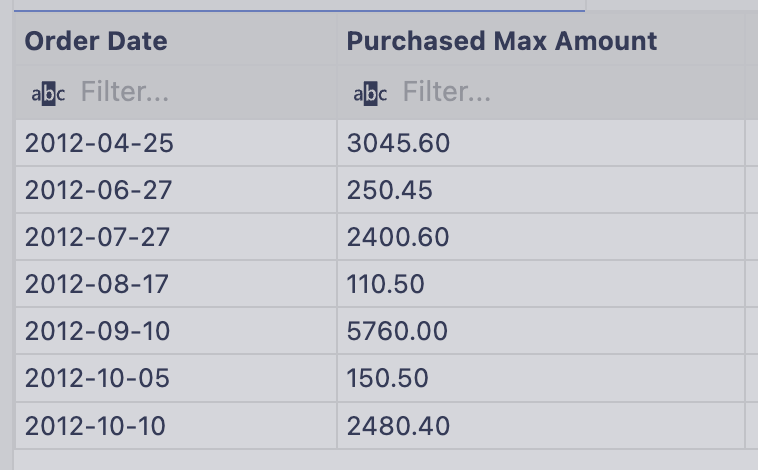
\includegraphics[width=.8\linewidth]{images/output/q5.png}
        \caption*{Products sold in 2003 but not 2004.}
        \label{fig:q5}
    \end{subfigure}
    \begin{subfigure}{.5\textwidth}
        \centering
        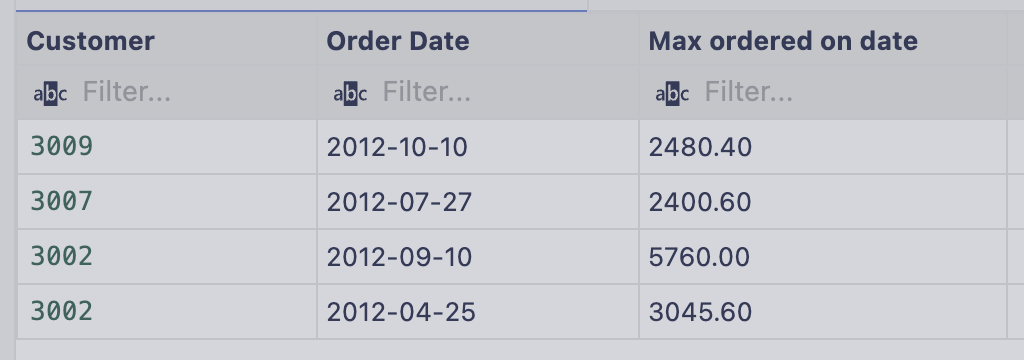
\includegraphics[width=.65\linewidth]{images/output/q7.png}
        \caption*{Names of products sold at less than 80\% of the MSRP.}
        \label{fig:q7}
    \end{subfigure}
\end{figure}


\end{document}